\chapter{Unsupervised Learning}
\label{ch:unsup}
Without labels there is no test accuracy to hide behind, so interviewers ask about mechanics and
assumptions: when does $k$-means stop, why does it need $k$ and scaling, what does EM actually
alternate, why standardise before PCA. OA papers favour the $k$-means stopping question and the PCA
scaling question; both are answered here with numbers.

\section{\texorpdfstring{$k$}{k}-means}
\prototype{Seven points, two starting centroids, one assign-and-update step by hand.}

\subsection{Lloyd's algorithm}
$k$-means seeks centroids $\bmu_1,\dots,\bmu_k$ and an assignment $c(i)$ minimising the
\vocab{inertia} (within-cluster sum of squares)
\[ J=\sum_i\norm{\x_i-\bmu_{c(i)}}^2. \]
Lloyd's algorithm alternates two steps, each of which minimises $J$ over one block of variables with
the other fixed:
\begin{enumerate}
	\ii \textbf{Assign}: $c(i)=\argmin_k\norm{\x_i-\bmu_k}$ (best $c$ for fixed $\bmu$).
	\ii \textbf{Update}: $\bmu_k=$ mean of points assigned to $k$ (the minimiser of
	$\sum_{c(i)=k}\norm{\x_i-\bmu}^2$ for fixed $c$).
\end{enumerate}

\begin{example}[One iteration by hand]
	Initial centroids $(1,1)$ and $(5,7)$:
	\begin{center}
		\small
		\begin{tabular}{cccc}
			\toprule
			point & distance to $\bmu_1$ & distance to $\bmu_2$ & cluster \\ \midrule
			\gv{c11_unsup/km_rows}
			\bottomrule
		\end{tabular}
	\end{center}
	New centroids are the cluster means: $\gv{c11_unsup/km_c1}$ (\code{KMeans(max_iter=1)} agrees).
	Inertia over the iterations: $\gv{c11_unsup/km_inertia}$, converged after
	$\gv{c11_unsup/km_iters}$ assignment passes.
\end{example}

\subsection{Why it stops, and the stopping conditions}
Each step cannot increase $J$, $J\ge0$, and there are finitely many assignments, so Lloyd's algorithm
terminates --- at a \emph{local} minimum, not necessarily the global one (which is NP-hard to find).
In practice it stops when any of these holds:
\begin{itemize}
	\ii no point changes cluster (assignments are stable --- the classical criterion);
	\ii centroids move less than a tolerance (scikit-learn: \code{tol} on the centroid shift);
	\ii the decrease in inertia falls below a threshold;
	\ii a maximum number of iterations (\code{max_iter}) is reached.
\end{itemize}

\begin{remark}
	\trap ``$k$-means stops when the inertia reaches zero'' (only if $k=n$) or ``when every cluster has
	the same number of points'' (never a criterion). Also, $k$-means always converges but may converge to
	a poor local optimum: hence multiple restarts (\code{n_init}) and smart seeding.
\end{remark}

\begin{figure}[ht]
	\centering
	\begin{tikzpicture}
		\begin{axis}[napkinplot, width=0.6\linewidth, height=0.45\linewidth, grid=none,
				xlabel=$x_1$, ylabel=$x_2$]
			\addplot[scatter, only marks, mark=*, mark size=1pt, point meta=\thisrow{c},
				colormap={km}{color=(blue!45) color=(red!45) color=(ForestGreen!45)}] table[x=x,y=y] {gen/ml/data/c11_unsup-blobs.dat};
			\foreach \k in {0,1,2}{
				\addplot[black, thick, -Stealth, mark=square*, mark size=1.6pt] table[x=x,y=y] {gen/ml/data/c11_unsup-traj\k.dat};}
		\end{axis}
	\end{tikzpicture}
	\caption{Lloyd iterations from a deliberately bad start (all three centroids inside one blob). The
		centroids (squares) walk to the cluster centres; inertia decreases at every step.}
	\label{fig:kmeans-traj}
\end{figure}

\subsection{Initialisation: \texorpdfstring{$k$}{k}-means++}
\vocab{$k$-means++} \cite{kmeanspp} picks the first centroid uniformly at random, then each next one
with probability proportional to $D(\x)^2$, the squared distance to the nearest centroid already chosen.
It spreads the seeds out and comes with an $O(\log k)$ approximation guarantee in expectation. On 8
well-separated blobs, single runs with random initialisation ended more than 5\% above the best inertia
found in $\gv{c11_unsup/rand_bad}$ of 50 seeds (worst run $\gv{c11_unsup/rand_worst}\times$ the best);
with $k$-means++ in $\gv{c11_unsup/pp_bad}$ (worst $\gv{c11_unsup/pp_worst}\times$).

\subsection{Choosing \texorpdfstring{$k$}{k}; assumptions}
Inertia always decreases with $k$, so look for an \vocab{elbow}, or use the \vocab{silhouette}: for
point $i$ with mean intra-cluster distance $a(i)$ and mean distance $b(i)$ to the nearest other cluster,
$s(i)=\frac{b(i)-a(i)}{\max(a(i),b(i))}\in[-1,1]$. For $(0,0)$ in clusters
$\{(0,0),(0,1),(1,0)\}$ and $\{(5,5),(5,6),(6,5)\}$: $a=\gv{c11_unsup/sil_a}$, $b=\gv{c11_unsup/sil_b}$,
$s=\gv{c11_unsup/sil_s}$ (matches \code{silhouette_samples}). On four blobs the mean silhouette peaks at
$k=\gv{c11_unsup/sil_best_k}$.

\begin{center}
	\begin{tikzpicture}
		\begin{groupplot}[group style={group size=2 by 1, horizontal sep=1.4cm},
				width=0.45\linewidth, height=0.3\linewidth, grid=major, grid style={gray!20},
				axis lines=left, xlabel={$k$}, ticklabel style={font=\scriptsize}]
			\nextgroupplot[ylabel={inertia}]
			\addplot[blue!80!black, thick, mark=*, mark size=1.2pt] table[x=k,y=inertia] {gen/ml/data/c11_unsup-elbow.dat};
			\nextgroupplot[ylabel={mean silhouette}]
			\addplot[red!80!black, thick, mark=square*, mark size=1.2pt] table[x=k,y=sil] {gen/ml/data/c11_unsup-elbow.dat};
		\end{groupplot}
	\end{tikzpicture}
\end{center}

$k$-means implicitly assumes spherical clusters of similar size and spread (it is EM for a Gaussian
mixture with equal, isotropic, vanishing variances). It uses Euclidean distance, so features must be
scaled; it is sensitive to outliers (means are not robust --- $k$-medoids uses actual points); and it
cannot find non-convex shapes (\Cref{fig:moons-db}).

\section{Hierarchical clustering}
\prototype{Five numbers $1,2,4,7,11$ merged bottom-up under three linkages.}
\vocab{Agglomerative} clustering starts with singletons and repeatedly merges the two closest clusters;
the history is a \vocab{dendrogram}, cut at any height to get a flat clustering --- no $k$ needed in
advance. Distance between clusters (\vocab{linkage}): \emph{single} (closest pair; finds chains,
suffers from ``chaining''), \emph{complete} (farthest pair; compact clusters), \emph{average} (mean
pairwise), \emph{Ward} (smallest increase in within-cluster variance; closest in spirit to $k$-means).

\begin{example}[Merge heights]
	For $1,2,4,7,11$: single linkage merges at heights $\gv{c11_unsup/hc_single}$ ($\{1,2\}$, then $4$
	joins at distance $2$, then $7$ at $3$, then $11$ at $4$); complete linkage at
	$\gv{c11_unsup/hc_complete}$; average linkage at $\gv{c11_unsup/hc_average}$ (all three match
	\code{scipy.cluster.hierarchy.linkage}).
\end{example}
\begin{center}
	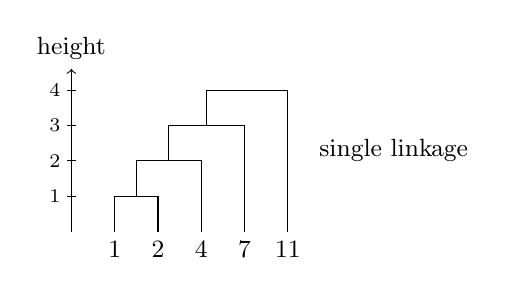
\begin{tikzpicture}[x=0.55cm, y=0.45cm, font=\small]
		\foreach \x/\l in {0/1,1/2,2/4,3/7,4/11} \node[below] at (\x,0) {\l};
		\draw (0,0) -- (0,1) -- (1,1) -- (1,0);
		\draw (0.5,1) -- (0.5,2) -- (2,2) -- (2,0);
		\draw (1.25,2) -- (1.25,3) -- (3,3) -- (3,0);
		\draw (2.125,3) -- (2.125,4) -- (4,4) -- (4,0);
		\draw[->] (-1,0) -- (-1,4.6) node[above] {height};
		\foreach \h in {1,2,3,4} \draw (-1.1,\h) -- (-0.9,\h) node[left=2pt] {\scriptsize\h};
		\node[right] at (4.5,2.3) {single linkage};
	\end{tikzpicture}
\end{center}
Cost: naive agglomeration is $O(n^3)$ time and $O(n^2)$ memory for the distance matrix, so it is used on
thousands, not millions, of points.

\section{DBSCAN}
\prototype{Two interleaved half-moons that $k$-means cuts in half.}
\vocab{DBSCAN} \cite{dbscan} groups points in dense regions. With radius $\varepsilon$ and threshold
\code{min_samples}: a \vocab{core point} has at least \code{min_samples} points (itself included) within
$\varepsilon$; a \vocab{border point} is within $\varepsilon$ of a core point but is not core; everything
else is \vocab{noise}. Clusters are connected components of core points plus their borders.
\begin{example}[Labelling points]
	Points $(0,0),(0,1),(1,0),(1,1),(2.2,1),(5,5)$, $\varepsilon=1.5$, \code{min_samples}$=4$.
	Neighbour counts: $\gv{c11_unsup/db_counts}$, so the kinds are \gv{c11_unsup/db_kinds}.
\end{example}
Strengths: arbitrary shapes, number of clusters not specified, explicit noise. Weaknesses: one global
density threshold (clusters of different densities break it --- HDBSCAN and OPTICS address this),
choosing $\varepsilon$ (look at the sorted distance to the $k$-th neighbour), and high dimensions.
On two moons, $k$-means reaches adjusted Rand index $\gv{c11_unsup/ari_km}$ and DBSCAN
$\gv{c11_unsup/ari_db}$.

\begin{figure}[ht]
	\centering
	\begin{tikzpicture}
		\begin{groupplot}[group style={group size=2 by 1, horizontal sep=0.6cm},
				width=0.5\linewidth, height=0.36\linewidth, ticklabel style={font=\scriptsize},
				title style={font=\small}]
			\nextgroupplot[title={$k$-means, $k=2$}]
			\addplot[scatter, only marks, mark=*, mark size=0.9pt, point meta=\thisrow{c},
				colormap={rb}{color=(blue!70) color=(red!70)}] table[x=x,y=y] {gen/ml/data/c11_unsup-moons_km.dat};
			\nextgroupplot[title={DBSCAN, $\varepsilon=0.2$}, yticklabels={}]
			\addplot[scatter, only marks, mark=*, mark size=0.9pt, point meta=\thisrow{c},
				colormap={rb}{color=(blue!70) color=(red!70)}] table[x=x,y=y] {gen/ml/data/c11_unsup-moons_db.dat};
		\end{groupplot}
	\end{tikzpicture}
	\caption{$k$-means draws a straight boundary between two centroids; DBSCAN follows density.}
	\label{fig:moons-db}
\end{figure}

\section{Gaussian mixtures and EM}
\prototype{A histogram with two bumps: estimate both bumps without knowing which point came from which.}

\subsection{The model and the difficulty}
A \vocab{Gaussian mixture} has density $p(\x)=\sum_k\pi_k\Normal(\x;\bmu_k,\bSigma_k)$. If we knew each
point's component $z_i$, fitting would be per-component MLE; we do not, and the log-likelihood
$\sum_i\log\sum_k\pi_k\Normal(\x_i;\bmu_k,\bSigma_k)$ has a sum inside the log with no closed-form
maximiser.

\subsection{EM}
\vocab{Expectation--maximisation} \cite{dempster1977} alternates:
\begin{itemize}
	\ii \textbf{E-step}: compute \vocab{responsibilities}
	\[ r_{ik}=\Prob(z_i=k\mid\x_i)=\frac{\pi_k\Normal(\x_i;\bmu_k,\bSigma_k)}{\sum_j\pi_j\Normal(\x_i;\bmu_j,\bSigma_j)}. \]
	\ii \textbf{M-step}: re-estimate with soft counts $N_k=\sum_ir_{ik}$:
	$\pi_k=N_k/n$, $\bmu_k=\frac1{N_k}\sum_ir_{ik}\x_i$,
	$\bSigma_k=\frac1{N_k}\sum_ir_{ik}(\x_i-\bmu_k)(\x_i-\bmu_k)\T$.
\end{itemize}
\begin{proof}[Why it works]
	For any distribution $q$ over $z$, Jensen's inequality gives
	\[ \log p(\x)=\log\sum_zq(z)\frac{p(\x,z)}{q(z)}\ge\sum_zq(z)\log\frac{p(\x,z)}{q(z)}, \]
	a lower bound (the ELBO) with gap $\KL(q\,\|\,p(z\mid\x))$. The E-step sets $q=p(z\mid\x)$, making the bound tight; the
	M-step maximises the bound over the parameters. So the likelihood never decreases: it is coordinate
	ascent on the ELBO, converging to a local maximum or saddle.
\end{proof}
\codefile[code/ml/c11\_unsup.py: one EM step for a 1-D mixture]{gen/ml/snip/c11_unsup-em.py}

\begin{example}[EM, checked]
	Equal weights, means $-1$ and $1$, unit variances: for $x=-1,0,2$ the responsibilities of the
	first component are $(\gv{c11_unsup/e_resp})$ --- a point midway gets $0.5$. On 500 points drawn from
	$0.6\,\Normal(-2,0.8^2)+0.4\,\Normal(2.5,1.2^2)$, EM converges in $\gv{c11_unsup/em_iters}$ iterations to
	$\gv{c11_unsup/em_params}$, identical to scikit-learn's \code{GaussianMixture} started from the same
	point; the log-likelihood rises at every iteration.
\end{example}

$k$-means is the ``hard'' limit: responsibilities rounded to 0/1, all covariances $\sigma^2\I$ with
$\sigma\to0$. GMMs give soft assignments, elliptical clusters, and a density usable for anomaly
detection; choose $k$ with BIC (\Cref{ch:eval}). Pitfalls: a component can collapse onto one point
(variance $\to0$, likelihood $\to\infty$), hence a small \code{reg_covar}; and EM is sensitive to
initialisation (usually from $k$-means).

\section{PCA}
\prototype{Ten 2-D points that lie near a line: one number per point keeps 96\% of the variance.}

\subsection{Two derivations}
\textbf{Maximum variance.} Find the unit vector $\uu$ maximising the variance of the projections of
centred data, $\uu\T\mathbf S\uu$ with $\mathbf S$ the sample covariance, subject to $\uu\T\uu=1$. The
Lagrangian $\uu\T\mathbf S\uu-\lambda(\uu\T\uu-1)$ gives $\mathbf S\uu=\lambda\uu$: $\uu$ is an
eigenvector and the variance achieved is $\lambda$, so take the top eigenvector. Each next component
is the top eigenvector orthogonal to the previous ones.

\textbf{Minimum reconstruction error / SVD.} With centred $\X=\U\bSigma\V\T$, the best rank-$k$
approximation (Eckart--Young, \Cref{ch:maths}) uses the top $k$ right singular vectors, which are the
eigenvectors of $\X\T\X=(n-1)\mathbf S$, and $\lambda_j=\sigma_j^2/(n-1)$. Libraries use the SVD: it never
forms $\X\T\X$ and is more stable.

\begin{example}[PCA by hand]
	Ten points with mean $(\gv{c11_unsup/pca_mean})$ and covariance
	$\mathbf S=\begin{psmallmatrix}\gv{c11_unsup/pca_S}\end{psmallmatrix}$. Its eigenvalues are
	$\gv{c11_unsup/pca_l1}$ and $\gv{c11_unsup/pca_l2}$; PC1 $=(\gv{c11_unsup/pca_v1})$ explains
	$\gv{c11_unsup/pca_evr}$ of the variance. The first point $(2.5,2.4)$ projects to
	$z_1=(2.5-1.81,\,2.4-1.91)\cdot\text{PC1}=\gv{c11_unsup/pca_z}$. Eigenvalues, PC1 (up to sign) and the
	projection match \code{sklearn.decomposition.PCA}, and equal $\sigma_j^2/(n-1)$ from the SVD.
\end{example}

\subsection{Why standardise first}
PCA maximises \emph{variance}, which depends on units. In the wine data, \texttt{proline} has variance
$\gv{c11_unsup/wine_var_proline}$ while \texttt{hue} has $\gv{c11_unsup/wine_var_hue}$. Unscaled, PC1
explains $\gv{c11_unsup/wine_evr_raw}$ of the variance and is essentially the
\texttt{\gv{c11_unsup/wine_top_raw}} axis (loading $\gv{c11_unsup/wine_load_raw}$) --- a unit
conversion, not structure. After standardising, PC1 explains $\gv{c11_unsup/wine_evr_std}$, 8 components
reach 90\%, and $k$-means on the first two components recovers the wine cultivars with adjusted Rand
index $\gv{c11_unsup/wine_ari_std}$ versus $\gv{c11_unsup/wine_ari_raw}$ unscaled.

\begin{remark}
	\trap ``Always standardise before PCA'' is the expected answer when features have different units;
	the precise answer is: standardise when variance differences are artefacts of units (PCA on the
	correlation matrix); do not, when all features share a unit and their variances are meaningful (pixel
	intensities, returns on similar assets). And always \emph{centre}. Other traps: PCA is unsupervised,
	so the top components need not be the most predictive; it is linear; and the components are only
	defined up to sign.
\end{remark}
Choose $k$ by cumulative explained variance (e.g.\ 90--95\%), a scree-plot elbow, or downstream
validation score. Uses: compression, de-noising, visualisation, decorrelating features for linear
models (PCA regression), speeding up distance-based methods.

\section{ICA, t-SNE and UMAP}
\prototype{Two speakers recorded by two microphones: unmix the voices.}
\vocab{Independent component analysis} assumes $\x=\A\bm s$ with \emph{statistically independent,
	non-Gaussian} sources $\bm s$ and finds an unmixing matrix maximising non-Gaussianity (FastICA uses
negentropy approximations). PCA only decorrelates (second-order statistics) and cannot recover the sources;
mixing a square wave and a sine wave, ICA recovers both with correlation at least
$\gv{c11_unsup/ica_corr}$ while PCA's best match is only $\gv{c11_unsup/pca_corr}$. ICA recovers sources up to
order and scale, and fails for Gaussian sources (any rotation of independent Gaussians is still
independent).

\vocab{t-SNE} \cite{tsne} turns pairwise distances into neighbour probabilities (Gaussian in input space,
with bandwidths set by a \emph{perplexity}, roughly the effective number of neighbours) and finds a 2-D
embedding whose Student-$t$ neighbour probabilities match them, minimising a KL divergence. The heavy
tail lets moderately distant points spread out, which separates clusters. \vocab{UMAP} builds a fuzzy
$k$-NN graph and optimises a cross-entropy between graph and embedding; it is faster and often preserves
more global structure. For both: use for \emph{visualisation}; cluster sizes and inter-cluster distances in
the picture are not meaningful; results depend on perplexity/neighbours and the random seed; there is no
\code{transform} for new points in standard t-SNE.

\section{Anomaly detection}
\prototype{Ten scattered points among 300 normal ones: score how easy each is to isolate.}
\vocab{Isolation forest} \cite{isoforest} builds random trees by choosing a random feature and a random
threshold between its min and max, until each point is alone. Anomalies are few and different, so they are
isolated near the root: short average path length $h(\x)$. The score is $2^{-\E[h(\x)]/c(n)}$ with
$c(n)=2H(n-1)-2(n-1)/n$ the average path length of an unsuccessful binary-search-tree lookup
($c(256)=\gv{c11_unsup/iso_c256}$ for the default sub-sample of 256). On our data the 10 planted outliers
average score $\gv{c11_unsup/iso_out_mean}$ against $\gv{c11_unsup/iso_in_mean}$ for inliers, and all
$\gv{c11_unsup/iso_top10_hits}$ of the 10 highest scores are planted outliers. Alternatives: GMM density
(low likelihood), one-class SVM, local outlier factor (density relative to neighbours), reconstruction error of
PCA or an autoencoder.

\section{Association rules}
\prototype{Six shopping baskets: does buying butter predict buying bread?}
For itemsets $A,B$ over $N$ transactions:
\begin{gather*}
	\mathrm{support}(A)=\frac{\#\{t: A\subseteq t\}}{N},\qquad
	\mathrm{confidence}(A\Rightarrow B)=\frac{\mathrm{support}(A\cup B)}{\mathrm{support}(A)},\\
	\mathrm{lift}(A\Rightarrow B)=\frac{\mathrm{confidence}(A\Rightarrow B)}{\mathrm{support}(B)}.
\end{gather*}
\begin{example}[Baskets]
	Transactions: \{bread, milk\}, \{bread, butter, milk\}, \{bread, butter\}, \{milk, tea\}, \{bread, butter,
	milk\}, \{bread, tea\}. Support(bread) $=\gv{c11_unsup/sup_bread}$, support(butter) $=\gv{c11_unsup/sup_butter}$,
	support(bread, butter) $=\gv{c11_unsup/sup_bb}$. Confidence(butter $\Rightarrow$ bread)
	$=\gv{c11_unsup/conf_butter_bread}$, but confidence(bread $\Rightarrow$ butter) $=\gv{c11_unsup/conf_bread_butter}$:
	confidence is not symmetric. Lift (symmetric) $=\gv{c11_unsup/lift_bb}>1$: positively associated;
	lift(milk, tea) $=\gv{c11_unsup/lift_mt}<1$.
\end{example}
\vocab{Apriori} \cite{apriori} finds frequent itemsets level by level using \emph{anti-monotonicity}: every
subset of a frequent itemset is frequent, so a candidate with an infrequent subset is pruned without
counting. With minimum support $1/3$ it returns \gv{c11_unsup/freq_sets} --- the same as brute-force
enumeration.

\begin{remark}
	\trap High confidence alone is misleading when the consequent is common: ``anything $\Rightarrow$
	bread'' has high confidence because 83\% of baskets contain bread. Lift corrects for this; lift $=1$
	means independence.
\end{remark}

\begin{moral}
	$k$-means is coordinate descent on inertia (it always stops, maybe badly); EM is coordinate ascent on a
	likelihood bound; PCA is an eigenproblem on the covariance --- so scale before it unless units agree.
\end{moral}

\section\problemhead

\begin{problem}[One \texorpdfstring{$k$}{k}-means step]
	\onechili
	1-D points $1,2,3,8,9,10,25$ with initial centroids $2$ and $9$. Do one assignment and update. What
	happens next, and what would $k$-means with $k=2$ do to the outlier $25$?
	\begin{hint}
		$25$ is closer to $9$.
	\end{hint}
	\begin{sol}
		Clusters $\{1,2,3\}$ and $\{8,9,10,25\}$; new centroids $\gv{c11_problems/p11a_c1}$ and
		$\gv{c11_problems/p11a_c2}$. Next assignment is unchanged ($8$ is closer to $13$ than to $2$), so it has
		converged. The outlier drags its centroid from $9$ to $13$; $k$-medians or $k$-medoids would resist.
	\end{sol}
\end{problem}

\begin{problem}[PCA explained variance]
	\onechili
	A covariance matrix has eigenvalues $4.0$, $2.5$, $1.0$, $0.3$, $0.2$. How many components keep at least 90\%
	of the variance? What fraction does PC1 explain?
	\begin{hint}
		Total variance is the trace, the sum of the eigenvalues.
	\end{hint}
	\begin{sol}
		Total $8.0$. Cumulative fractions: $0.5$, $0.8125$, $0.9375$, \dots, so 3 components. PC1 explains
		$\gv{c11_problems/p11b_pc1}$.
	\end{sol}
\end{problem}

\begin{problem}[PCA of a $2\times2$ covariance]
	\twochili
	Centred data have covariance $\begin{psmallmatrix}3&1\\1&3\end{psmallmatrix}$. Find the principal
	directions, the variances along them, and the projection of $\x=(2,0)$ onto PC1.
	\begin{hint}
		Eigenvectors of $\begin{psmallmatrix}a&b\\b&a\end{psmallmatrix}$ are $(1,\pm1)/\sqrt2$.
	\end{hint}
	\begin{sol}
		Eigenvalues $4$ (direction $(1,1)/\sqrt2$) and $2$ (direction $(1,-1)/\sqrt2$). PC1 explains
		$2/3$. Projection: $(2,0)\cdot(1,1)/\sqrt2=\sqrt2=\gv{c11_problems/p11c_z}$.
	\end{sol}
\end{problem}

\begin{problem}[Association rule]
	\onechili
	In 1000 orders, 200 contain chips, 300 contain cola, 120 contain both. Compute support, confidence of
	chips $\Rightarrow$ cola, and lift. Is the rule useful?
	\begin{hint}
		Lift $=\Prob(\text{both})/(\Prob(\text{chips})\Prob(\text{cola}))$.
	\end{hint}
	\begin{sol}
		Support $0.12$; confidence $120/200=0.6$; lift $0.6/0.3=\gv{c11_problems/p11d_lift}$. Customers who
		buy chips are twice as likely as average to buy cola: a useful rule for placement or bundling.
	\end{sol}
\end{problem}

\begin{problem}[EM responsibility]
	\twochili
	A 1-D mixture has $\pi=(0.3,0.7)$, means $0$ and $4$, both variances $1$. Compute the responsibility of
	component 1 for $x=1.5$.
	\begin{hint}
		Ratio of $\pi_k\phi(x-\mu_k)$; the normalising constants cancel.
	\end{hint}
	\begin{sol}
		$0.3e^{-1.125}$ versus $0.7e^{-3.125}$; $r_1=\frac{0.3e^{-1.125}}{0.3e^{-1.125}+0.7e^{-3.125}}=
			\gv{c11_problems/p11e_r}$. Although $x$ is closer to $0$ than to $4$ by a wide margin, the larger prior
		of component 2 is not enough to win.
	\end{sol}
\end{problem}
